
\section{Empirical Evaluation}
\label{sec:experitns}

% \begin{table}[t]
%    \vspace{-2mm}
% \scriptsize
% \centering
% \caption{\textbf{Token Generation Latency} Average per-token latency (ms) with batch size 1 on 8xA100 80GB with NVLink
%   when generating sequences with prompt lengths 128, 256, 512, and 1024, using
%   fp16 precision. Across
%   the board, \name{} speeds up generation by 1.8-2.5$\times$ compared to the
%   state-of-the-art FT and by 4.8-6.8$\times$ compared to the widely used
%   HF implementation.}
%   \vspace{2mm}
% \resizebox{0.9\linewidth}{!}{ \centering \Huge \begingroup
%   \setlength{\tabcolsep}{10pt} \renewcommand{\arraystretch}{1.3}
% \begin{tabular}{c|c|c|c|c}
% \toprule
%  Sequence length             & 128           & 256           & 512           & 1024	\\
% \hline
%  OPT-175B Hugging Face       & 107.9         & 108.0         & 110.4         & 112.7 \\
%  OPT-175B FasterTransformer & 40.5          & 40.9          & 41.7          & 43.4 \\
%  DejaVu-OPT-175B (ours)      & \color{red}{Update \textbf{15.9}} & \color{red}{\textbf{17.1}} & \color{red}{\textbf{19.8}} & \color{red}{\textbf{23.6}}  \\
%  \bottomrule
% \end{tabular}
% \endgroup
% }
% \label{table:main_latency}
% \vspace{-2mm}
% %%Zhao: Someone comment out the above label and table. However, we actually refer to this label somewhere in the paper, please see the warning.
% \end{table}

\begin{figure}[]
  \centering
    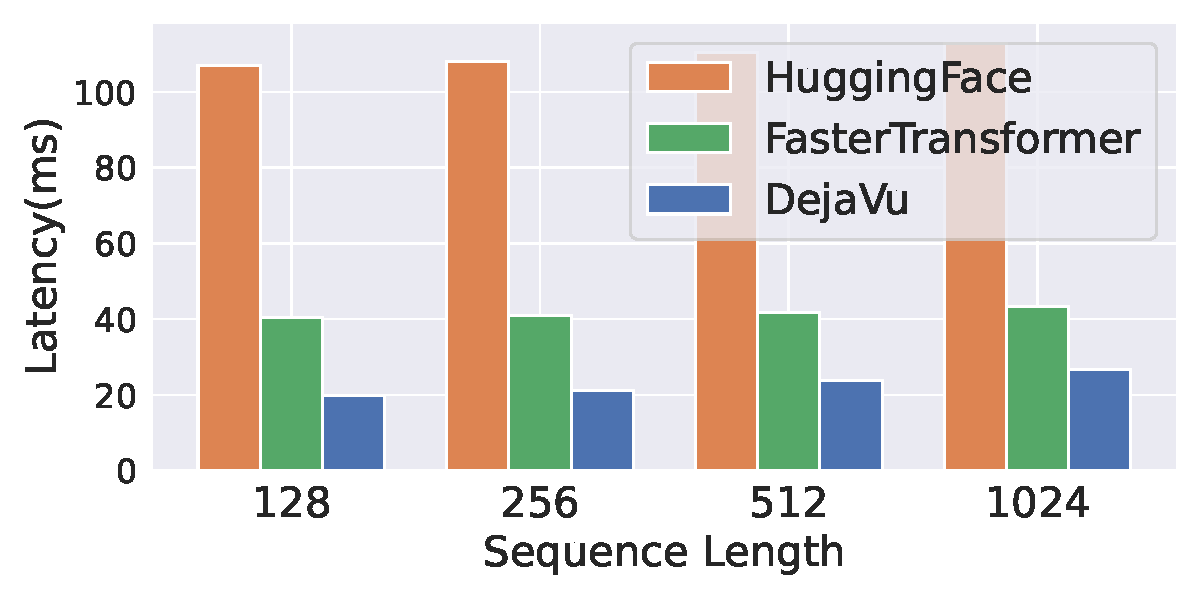
\includegraphics[width=0.38\textwidth]{figure/experiment/sequence_speed_up_ms.pdf}
    \vspace{-6mm}
  % \caption{ Average per-token latency speed up on 8 A100 80GB when generating with various sequence length using FP16. }
  \caption{Average per-token latency (ms) with batch size 1 on 8 A100-80GB with NVLink
  when generating sequences with prompt lengths 128, 256, 512, and 1024, using FP16. \name{} speeds up generation by 1.8-2$\times$ compared to the
  state-of-the-art FT and by 4.8-6$\times$ compared to the widely used
  HF implementation.}
  \label{table:main_latency} 
     \vspace{-4mm}
\end{figure}

\begin{table*}[t]
\scriptsize
\centering
\vspace{-3mm}
\caption{Accuracy of zero-shot tasks and language modeling when sparsifying the MLP block and the Attention block separately. The sparsity is set at 85\% for MLP-block and 50\% for Attention-block. \name{} incurs no accuracy drop across the boards.}
\vspace{2mm}
\resizebox{0.8\linewidth}{!}{
\centering
\Huge
\begingroup
\setlength{\tabcolsep}{10pt}
\renewcommand{\arraystretch}{1.2}
\begin{tabular}{c||ccccccc|cc}
\specialrule{.15em}{.05em}{.05em}
 Model & CB & COPA & Lambada & OpenBookQA & PIQA  & RTE & Winogrande  &  Wikitext & C4	\\
\cline{1-10}
 OPT-175B & 0.3523 &  0.86   &  0.7584 & 0.446 & 0.8096 & 0.6029 &  0.7261  & 10.8221 & 7.7224 \\
 \cline{1-10}
 \name{}-MLP-OPT-175B & 0.3544 & 0.85 & 0.7619 & 0.446 & 0.8096 &   0.6065 &  0.7206 &  10.7988 & 7.7393  \\
 \cline{1-10}
 \name{}-Attention-OPT-175B & 0.3544 & 0.86  & 0.7586 & 0.4460 & 0.8063 &   0.5921 &  0.7245 & 10.8696 & 7.7393  \\
\specialrule{.15em}{.05em}{.05em}
\end{tabular}
\endgroup
}
\vspace{-2mm}
\label{table:exp-mlp-accruacy}
\end{table*}
% \begin{table*}[t]
% \scriptsize
% \centering
% \vspace{-3mm}
% \caption{Accuracy of zero-shot tasks and language modeling when sparsifying the MLP block and the Attention block separately. The sparsity is set at 85\% for MLP-block and 50\% for Attention-block. \name{} incurs no accuracy drop across the boards.}
% \vspace{2mm}
% \resizebox{0.8\linewidth}{!}{
% \centering
% \Huge
% \begingroup
% \setlength{\tabcolsep}{10pt}
% \renewcommand{\arraystretch}{1.2}
% \begin{tabular}{c||cccccccc|cc}
% \specialrule{.15em}{.05em}{.05em}
%  Model & CB & COPA & Hellaswag & Lambada & OpenBookQA & PIQA  & RTE & Winogrande  &  Wikitext & C4	\\
% \cline{1-11}
% %  OPT-30B&  &  &  &  &  & &  &  &  &  &  & 	\\
% %  DejaVu-OPT-30B &  &  &  &  &  &  &  &   &  &  &  &   \\
% % \cline{1-13}
% %  OPT-66B& 0.3928 &  0.87 & 0.7400 & 0.7508 & 0.426 & 0.7921 &  0.6028 & 0.6890 & 0.5 & 0.5480 & 12.1988 & 	\\
% %  MLP-Sparse-OPT-66B & 0.4285 & 0.87  & 0.7416 & 0.7458 & 0.434 & 0.7933 & 0.5884 &  0.6898 & 0.5 & 0.5480 & 12.2703  &   \\
% % \cline{1-13}
%  OPT-175B & 0.3523 &  0.86 & 0.7814  &  0.7584 & 0.446 & 0.8096 & 0.6029 &  0.7261  & 10.8221 & 7.7224 \\
%  \name{}-MLP-OPT-175B & 0.3544 & 0.85 & 0.7806 & 0.7619 & 0.446 & 0.8096 &   0.6065 &  0.7206 &  10.7988 & 7.7393  \\
%  \name{}-Attention-OPT-175B & 0.3544 & 0.86 & 0.7819 & 0.7586 & 0.4460 & 0.8063 &   0.5921 &  0.7245 & 10.8696 & 7.7393  \\
% \specialrule{.15em}{.05em}{.05em}
% \end{tabular}
% \endgroup
% }
% \vspace{-2mm}
% \label{table:exp-mlp-accruacy}
% \end{table*}




In Section~\ref{sec:main_result}, we present the end-to-end results that show \name{} achieves over 2$\times$ reduction in token generation latency compared to the state-of-the-art FasterTransformer and over 6$\times$ compared to Hugging Face with no accuracy loss. In Section~\ref{sec:abalation_mlp_att}, we perform a list of ablation studies such as independent evaluation on the inference-time contextual sparsity of the MLP block and the Attention block (Details are presented in Section~\ref{sec:appendix-exp}). At last, we present the additional results to demonstrate the future possibility of sparsifying the entire LLMs via layer skipping in Section~\ref{sec:exp_skip_layer}. 


% \begin{table*}[]
% \scriptsize
% \centering
% \caption{ \textbf{Result on Attention Sparse Predictor} }
% \resizebox{\linewidth}{!}{
% \centering
% \Huge
% \begingroup
% \setlength{\tabcolsep}{10pt}
% \renewcommand{\arraystretch}{1.3}
% \begin{tabular}{c||cccccccc|cc}
% \specialrule{.15em}{.05em}{.05em}
%  Model & CB & COPA & Hellaswag & Lambada & OpenBookQA & PIQA  & RTE & Winogrande  &   Wikitext & C4	\\
%  % OPT-66B& 0.3928 &  0.87 & 0.7400 & 0.7508 & 0.426 & 0.7921 &  0.6028 & 0.6890 & 0.5 & 0.5480 & 12.1988 & 	\\
%  % MLP-Sparse-OPT-66B & 0. & 0.  & 0. & 0. & 0. & 0. & 0. &  0. & 0. & 0. &   &   \\
% \cline{1-11}
%  OPT-175B & 0.3523 &  0.86 & 0.7814  &  0.7584 & 0.446 & 0.8096 & 0.6029 &  0.7261 & 10.8221 & 7.7224 \\
%  Attention-Sparse-OPT-175B & 0.3544 & 0.86 & 0.7819 & 0.7586 & 0.4460 & 0.8063 &   0.5921 &  0.7245 & 10.8696 & 7.7393  \\
% \specialrule{.15em}{.05em}{.05em}
% \end{tabular}
% \endgroup
% }
% \label{table:exp-att-accruacy}
% \end{table*}


\subsection{End-to-End Result}
\label{sec:main_result}

\textbf{Experiment Setting:}
We compare the accuracy of \name{}-OPT against the original OPT model on two language modeling datasets Wiki-Text~\cite{merity2016pointer} and C4~\cite{2019t5} and seven few-shot downstream tasks: CB~\cite{Marneffe2019TheCI}, COPA~\cite{gordon-etal-2012-semeval}, Lambada~\cite{radford2019language}, OpenBookQA~\cite{OpenBookQA2018}, PIQA~\cite{Bisk2020}, RTE~\cite{giampiccolo-etal-2007-third}, Winogrande~\cite{ai2:winogrande}. 
We use lm-eval-harness~\cite{eval-harness} for zero-shot and five-shot tasks.  We collect training data for the sparsity predictor using 500 random data points from the C4 training dataset. Our experiments are conducted on NVIDIA A100 80GB GPU servers.

\textbf{No accuracy drop until 75\% sparsity: } In Figure~\ref{exp:kshot}, we present \name{}-OPT-175B's accuracy trend.  In a zero-shot setting, the average accuracy across tasks does not drop until 75\% sparsity. A similar trend can be observed for the five-shot setting, which verifies the model's ability for in-context learning.  This result is exceptionally encouraging given our observation in Figure~\ref{fig:sparsity-175}, where we could impose 85\% sparsity when allowed full computation. 

% \textbf{Over 2$\times$ latency reduction: } 
% Figure~\ref{fig:main_latency} presents the latency speed-up for the token generation with OPT-175B. The best performance is at batch size 1, where \name{} achieves over 2$\times$ speed up compared to the state-of-the-art FasterTransformers and over 6$\times$ compared to the widely used Hugging Face. Increasing the batch size means more MLP neurons and attention heads to activate. Surprisingly, this does not grow linearly with the batch size and thus we still observe significant speed-up.

% % In Table~\ref{fig:main_latency}, we present the latency for token generation . Across prompt lengths, \name{}-OPT-175B achieves significant speed up compared to our baselines. At around 75\% sparsity, \name{} speeds up generation by 1.8-2.5$\times$ compared to the state-of-the-art FasterTransformers\footnote{http://github.com/NVIDIA/FasterTransformer} and by 4.8-6.8$\times$ compared to the widely used Hugging Face implementation\footnote{http://github.com/huggingface/transformers}. 

\textbf{Over 2$\times$ latency reduction: } 
Figure~\ref{table:main_latency} presents the latency speed-up for the token generation with OPT-175B at batch size 1, where \name{} achieves the best performance. At around 75\% sparsity, \name{} speeds up generation by 1.8-2$\times$ compared to the state-of-the-art FasterTransformers (FT)\footnote{http://github.com/NVIDIA/FasterTransformer} and by 4.8-6$\times$ to Hugging Face (HF) implementation\footnote{http://github.com/huggingface/transformers}. 






% \begin{table}[H]
%    \vspace{-2mm}

% \scriptsize
% \centering
% \caption{\textbf{Token Generation Latency} Average per-token latency (ms) with batch size 1 on 8xA100 80GB with NVLink
%   when generating sequences with prompt length 128, 256, 512, and 1024, using
%   fp16 precision.
%   For \name{}-OPT-175B, we set the MLP density to 10\% and attention density to
%   42\% (i.e., for each token, each GPU has on average 5 non-zero heads out of 12). Across
%   the board, \name{} speeds up generation by 1.8-2.5$\times$ compared to the
%   state-of-the-art FasterTransformer and by 4.8-6.8$\times$ compared to the widely used
%   Hugging Face implementation.}
%   \vspace{2mm}
% \resizebox{0.9\linewidth}{!}{ \centering \Huge \begingroup
%   \setlength{\tabcolsep}{10pt} \renewcommand{\arraystretch}{1.3}
% \begin{tabular}{c|c|c|c|c}
% \toprule
%  Sequence length             & 128           & 256           & 512           & 1024	\\
% \hline
%  OPT-175B Hugging Face       & 107.9         & 108.0         & 110.4         & 112.7 \\
%  OPT-175B FasterTransformer & 40.5          & 40.9          & 41.7          & 43.4 \\
%  DejaVu-OPT-175B (ours)      & \textbf{15.9} & \textbf{17.1} & \textbf{19.8} & \textbf{23.6}  \\
%  \bottomrule
% \end{tabular}
% \endgroup
% }
% \label{table:main_latency}
% %%Zhao: Someone comment out the above label and table. However, we actually refer to this label somewhere in the paper, please see the warning.
% \end{table}

\vspace{-2mm}
\subsection{Ablation Results}
\label{sec:abalation_mlp_att}

\textbf{Contextual Sparsity for Larger Batches:} Although this paper focuses on latency-sensitive settings, we demonstrate that \name{} generalizes to larger batches. we present the Union contextual sparsity (fraction of neurons/heads that are not used by any of the inputs in the batch) of different batches sizes for MLP and Attention blocks, respectively, in Figure~\ref{main:exp_sparsity_batch} and \ref{appendix:exp_sparsity_batch}. The union operation is essential to realize a fast sparse GEMM. Surprisingly the number of MLP neurons and Attention heads that \name{} activated does not grow linearly with the batch size. This suggests a power law distribution rather than a uniform distribution of parameter access from all input examples. This provides an opportunity for potentially extending Dejavu to the high-throughout setting. For example, we can first pre-process the inputs and batch similar inputs to enjoy a higher level of union contextual sparsity.

\textbf{Contextual sparsity on MLP blocks:} We study the contextual sparsification of the MLP block in OPT-175B. We leave the Attention block as dense computation. Table~\ref{table:exp-mlp-accruacy} shows the model performance at 85\% sparsity. The MLP sparse predictor introduces no accuracy loss on both zero-shot tasks and language modeling. In the training of the MLP sparse predictor, we observe that the sparse predictor achieves high validation accuracy. The shallow layer seems easier to model because the predictor has validation accuracy over 99\% in the shallow layers and drops to around 93\% in the ending layers. 

\textbf{Contextual sparsity on attention blocks:} In this section, we study the sparse predictor for the Attention block on OPT-175B and leave the MLP block as dense computation. Table~\ref{table:exp-mlp-accruacy} displays the test accuracy on zero-shot tasks and perplexity on the language modeling datasets. In summary, the Attention sparse predictor introduces no accuracy loss at around 50\% sparsity. During the training of the Attention sparse predictor, we observe different trends compared to the MLP sparse predictor. The validation accuracy is around 93\% in the middle layers and near 99\% in the shallow and deep layers.



\textbf{Contextual Sparsity on Smaller Models:} Our main experiments focus on OPT-175B. Here, we verify \name{}'s effectiveness on a smaller model, specifically OPT-66B. In Table~\ref{table:exp-66b-accuracy}, we summarize the accuracy on zero-shot task at $50\%$ 
sparsity. Similar to \name{}-OPT-175B, we notice no accuracy loss.

\textbf{Contextual Sparsity on Other Models:} We expand the evaluation to another model family. In Table~\ref{table:exp-bloom-accuracy}, we summarize the accuracy at attention sparsity 50\% and MLP sparsity 30\%. Similar to OPT family, we notice no accuracy loss. The lower sparsity level in MLP is due to the difference in activation function.

% \textbf{Compatibility with Quantization: } Following a similar setting in~\cite{frantar2023massive}, we test the compatibility of two orthogonal lines of efficient inference. We observe similar results when combined with 4-bit quantization; contextual sparsity can still preserve similar downstream task accuracy. 


\begin{table}[t]
\vspace{-4mm}
\scriptsize
\centering
\caption{\name{}-OPT66B on zero-shot downstream task.}
\vspace{2mm}
\resizebox{\linewidth}{!}{
\centering
\Huge
\begingroup
\setlength{\tabcolsep}{10pt}
\renewcommand{\arraystretch}{1.4}
\begin{tabular}{c||ccccccc}
\specialrule{.15em}{.05em}{.05em}
 Model & CB & COPA  & Lambada & OpenBookQA & PIQA  & RTE & Winogrande  	\\
\cline{1-8}
 OPT-66B& 0.3928 &  0.87  & 0.7508 & 0.426 & 0.7921 &  0.6028 & 0.6890 	\\
\cline{1-8}
\name{}-OPT-66B & 0.4285 & 0.87  & 0.7458 & 0.434 & 0.7933 & 0.5884 &  0.6898 \\
\cline{1-8}
\specialrule{.15em}{.05em}{.05em}
\end{tabular}
\endgroup
}
\vspace{-3mm}
\label{table:exp-66b-accuracy}
\end{table}




\iffalse

%%%Zhao: THe following table for some reason keeps generating compiling error. I retype everything again.
\begin{table}[t]
\vspace{-2mm}
\scriptsize
\centering
\caption{\name{}-BLOOM on zero-shot downstream task.
}\label{table:exp-bloom-accuracy}
\vspace{2mm}
\resizebox{\linewidth}{!}{
\centering
\Huge
\begingroup
\setlength{\tabcolsep}{10pt}
\renewcommand{\arraystretch}{1.3}
\begin{tabular}{c||cccccccc}
\specialrule{.15em}{.05em}{.05em}
             & CB    & COPA & OpenBookQA & PIQA  & RTE   & Winogrande & lambada \\
\cline{1-8}
BLOOM & 0.455 & 0.8  & 0448       & 0.79  & 0.617 & 0.704 & 0.677 \\
\cline{1-8}
Dejavu-BLOOM & 0.448 & 0.8  & 0.44       & 0.787 & 0.606 & 0.710    & 0.675      
\cline{1-8}
\specialrule{.15em}{.05em}{.05em}
\end{tabular}
\endgroup
}
\vspace{-1mm}
\end{table}
\fi

\begin{table}[t]
\vspace{-2mm}
\scriptsize
\centering
\caption{\name{}-BLOOM on zero-shot downstream task.}
\vspace{2mm}
\resizebox{\linewidth}{!}{
\centering
\Huge
\begingroup
\setlength{\tabcolsep}{10pt}
\renewcommand{\arraystretch}{1.4}
\begin{tabular}{c||ccccccc}
\specialrule{.15em}{.05em}{.05em}
 & CB    & COPA & OpenBookQA & PIQA  & RTE   & Winogrande & Lambada\\
 \cline{1-8}
BLOOM & 0.455 & 0.8  & 0448       & 0.79  & 0.617 & 0.704 & 0.677 \\
\cline{1-8}
Dejavu-BLOOM & 0.448 & 0.8  & 0.44       & 0.787 & 0.606 & 0.710    & 0.675      \\
\specialrule{.15em}{.05em}{.05em}
\end{tabular}
\endgroup
}
\vspace{-3mm}
\label{table:exp-bloom-accuracy}
\end{table}





\begin{figure}[t]
% \vspace{-2mm}
  \centering
     % \subfigure[MLP]{
    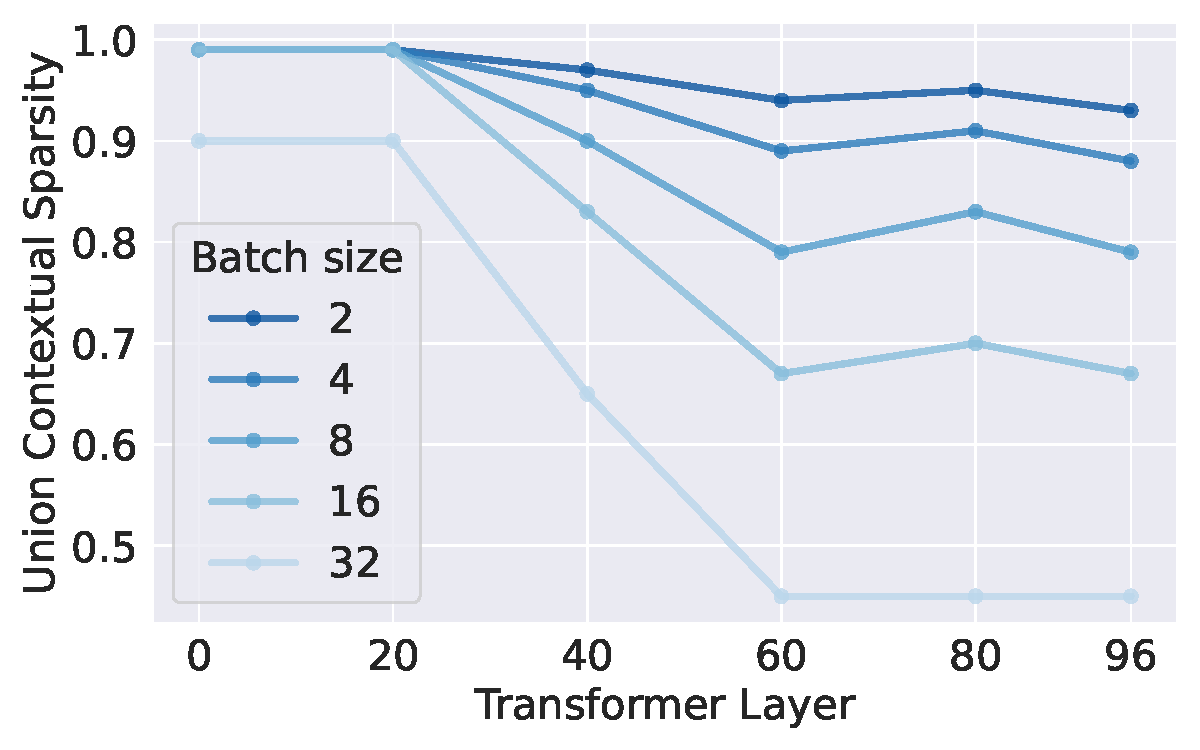
\includegraphics[width=0.36\textwidth]{figure/experiment/batch_sparsity_mlp.pdf}
    % }
   % \subfigure[Attention]{
   %  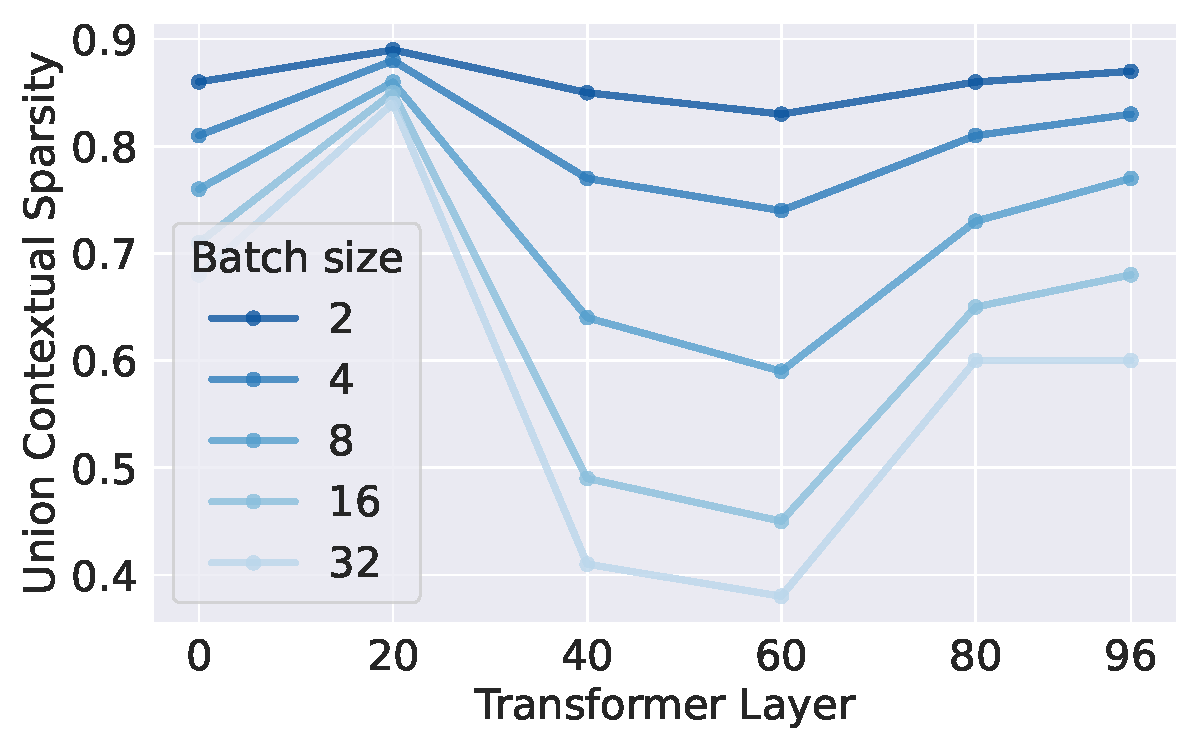
\includegraphics[width=0.40\textwidth]{figure/experiment/batch_sparsity_attention.pdf}
   %  }
   \vspace{-2mm}
  \caption{Union contextual sparsity with larger batch size.}
  \label{main:exp_sparsity_batch}
  \vspace{-2mm}
\end{figure}


\textbf{Non-Contextual Sparsity: } As we mentioned in Section~\ref{sec:introduction}, one could predict sparsity without contextual information. For non-contextual sparsity, we rely on the original embedding at the input layer. At every block, we first pass the original embedding to record a subset of parameters yielding a large norm. In the second pass, the embedding at every layer only uses the recorded subset. As shown in Figure~\ref{fig:contextual-static}, non-contextual prediction is not sufficient and leads to accuracy losses even at 50\% sparsity.  This result verifies our design choices of relying on the activation at every layer as input to make contextual sparsity predictions.

\textbf{Compatibility with Quantization:} Quantization is another promising direction for efficient language models. We investigate the possibility of combining contextual sparsity with quantization techniques. For \name{}-OPT-175B, we set the entire model sparsity at 75\%. For quantization, we apply 4-bit quantization on model weights (W4A16). As shown in Table~\ref{table:with-quantization}, the combination of quantization and \name{} almost always achieves better accuracy than \name{}  or quantization alone. This suggests that the approximation errors from these two directions do not get compounded. 
\begin{table}[t]
\vspace{-2mm}
\scriptsize
\centering
\caption{\name{}-OPT-175B with 4-bit quantization.}
\vspace{2mm}
\resizebox{\linewidth}{!}{
\centering
\Huge
\begingroup
\setlength{\tabcolsep}{10pt}
\renewcommand{\arraystretch}{1.4}
\begin{tabular}{c||ccccccc}
\specialrule{.15em}{.05em}{.05em}
 & CB    & COPA & OpenBookQA & PIQA  & RTE   & Winogrande & Lambada\\
 \cline{1-8}
OPT-175B                & 0.352 & 0.86 & 0.446      & 0.809 & 0.602 & 0.726      & 0.758           \\
\cline{1-8}
Dejavu-OPT-175B         & 0.402 & 0.85 & 0.450      & 0.802 & 0.592 & 0.726      & 0.753           \\
\cline{1-8}
OPT-175B + W4A16        & 0.356 & 0.85 & 0.44       & 0.806 & 0.574 & 0.714      & 0.757           \\
\cline{1-8}
Dejavu-OPT-175B + W4A16 & 0.365 & 0.86 & 0.452      & 0.805 & 0.592 & 0.726      & 0.754          \\
\specialrule{.15em}{.05em}{.05em}
\end{tabular}
\endgroup
}
\vspace{-3mm}
\label{table:with-quantization}
\end{table}